% TEXINPUTS=.:$HOME/git/bvtex: latexmk  -pdf <main>.tex
\documentclass[xcolor=dvipsnames]{beamer}

\input{defaults}
\input{beamer/preamble}

\setbeamertemplate{navigation symbols}{}
% \setbeamertemplate{background}[grid][step=1cm]

\usepackage{siunitx}
\usepackage{xmpmulti}
\usepackage[export]{adjustbox}
\usepackage{ulem}
\usepackage[outline]{contour}
\usepackage{pdfpages}
\usepackage{tikz}
\usepackage{tikzsymbols}
\usetikzlibrary{shapes.geometric, arrows}
\usetikzlibrary{positioning}

\definecolor{bvtitlecolor}{rgb}{0.98, 0.92, 0.84}
\definecolor{bvoutline}{rgb}{0.1, 0.1, 0.1}

\renewcommand{\bvtitleauthor}{Brett Viren}
\renewcommand{\bvtit}{simgraph}
\renewcommand{\bvtitle}{\LARGE Wire-Cell Toolkit\\Sim and Graph Updates\\Config and NF Integration}
\renewcommand{\bvevent}{{\small bnl-ub -- 2018-03-23}}
\renewcommand{\bvdate}{23 Mar 2018}
\renewcommand{\bvbeamerbackground}{}

\def\Put(#1,#2)#3{\leavevmode\makebox(0,0){\put(#1,#2){#3}}}

\begin{document}
\input{beamer/title.tex}
\input{beamer/toc.tex}


\section{New Stuff: Sim and Graph}
\begin{frame}
  \tableofcontents[currentsection,hideothersubsections]
\end{frame}

\begin{frame}
  \frametitle{New WCT Package: \texttt{pgraph}}
  The ``P'' could mean ``pipe'' or ``process''.
  \begin{itemize}\footnotesize
  \item Provides a \textbf{single-threaded} implementation of WCT's
    directed graph execution interface.
  \item Uses an invented ``ASAP'' graph execution model.
    \begin{itemize}\scriptsize
    \item[$\to$] Always execute the ``deepest'' graph nodes possible.
    \item Minimizes amount of ``in flight'' data (reduce memory usage).
    \item Note: \textbf{exactly wrong strategy} if multi-threaded:
      \begin{itemize}\scriptsize
      \item[$\to$] see \href{http://inspirehep.net/record/1503877}{I. Shapoval, thesis on GaudiHive}
      \end{itemize}
    \end{itemize}
  \item Finally, we can configure an \textbf{arbitrary graph of
      components}
    \begin{itemize}\scriptsize
    \item A new, generic ``app'' component: \texttt{Pgrapher} executes the graph.
    \item The \texttt{Fourdee} app is still left in the \texttt{gen} package.
    \item Hard-coded \texttt{Fourdee} C++ structure now can be
      expressed in configuration with help of a few new components.
    \end{itemize}
  \end{itemize}
\end{frame}


\begin{frame}
  \frametitle{New and Newish Components}
  In \texttt{gen}:
  \begin{description}\footnotesize
  \item[DepoMerger] merge two streams of deposition into one
    time-ordered stream (was hard-code C++ in \texttt{Fourdee}).
  \item[FrameSummer] add frames from two streams together \\ (also hard-coded in \texttt{Fourdee} C++).
  \item[BlipSource] a point-like deposition source of low, fixed
    energy or $^{39}$Ar spectrum, uniform vertices in a box.
  \item[TrackDespos] generate ideal, straight-line tracks in various ways (not new).
  \item[MultiDuctor] a rule-based switchyard managing other Ductors (newish).
  \end{description}
  In \texttt{sio}:
  \begin{description}\footnotesize
  \item[NumpyDepoSaver] save depos to Numpy array files.
  \item[NumpyFrameSaver] save frames to Numpy array files.
  \end{description}
  In \texttt{pgraph}:
  \begin{description}\footnotesize
  \item[Pgrapher] WCT app executing the graph
  \end{description}
\end{frame}

\section{Configuration}
\begin{frame}
  \tableofcontents[currentsection,hideothersubsections]
\end{frame}

\begin{frame}[fragile]
  \frametitle{\texttt{Pgrapher} Configuration Jsonnet file}
\scriptsize
\begin{verbatim}
local base_params = { 
  lar: {...}, detector: {...}, daq: {...}, adc: {...}, elec{...},
  sim: {noise: true, ...},
};
local uboone_params = base_params {...}; // also one for DUNE
local params = uboone_params;

local cosmics = {type: "TrackDepos", name: "cosmics", data: {...}};
local beam = {type: "TrackDepos", name: "beam", data: {...}};

local joincb = { type: "DepoMerger", name: "CosmicBeamJoiner" };
// ... more nodes defined

local app = { type:"Pgrapher", data: { edges: [
  {tail: {node: wc.tn(cosmics)}, head: {node: wc.tn(joincb), port:0}},
  {tail: {node: wc.tn(beam)}, head: {node: wc.tn(joincb), port:1}},
  // ...
]}};
[cosmics, beam, joincb, app, ...]  // resulting configuration sequence
\end{verbatim}
\end{frame}

\begin{frame}
  \frametitle{Noise+Signal and Just Signal}

  \vspace{-10mm}

  \begin{columns}
    \begin{column}{0.7\textwidth}
      \footnotesize
      Can switch noise on/off by drawing a different graph.
      \begin{itemize}\scriptsize
      \item Currently do it by editing the Jsonnet file.
      \item Switch could use Jsonnet's ``external variable'' feature.
      \end{itemize}
    \end{column}

    \begin{column}{0.3\textwidth}
      \begin{center}
        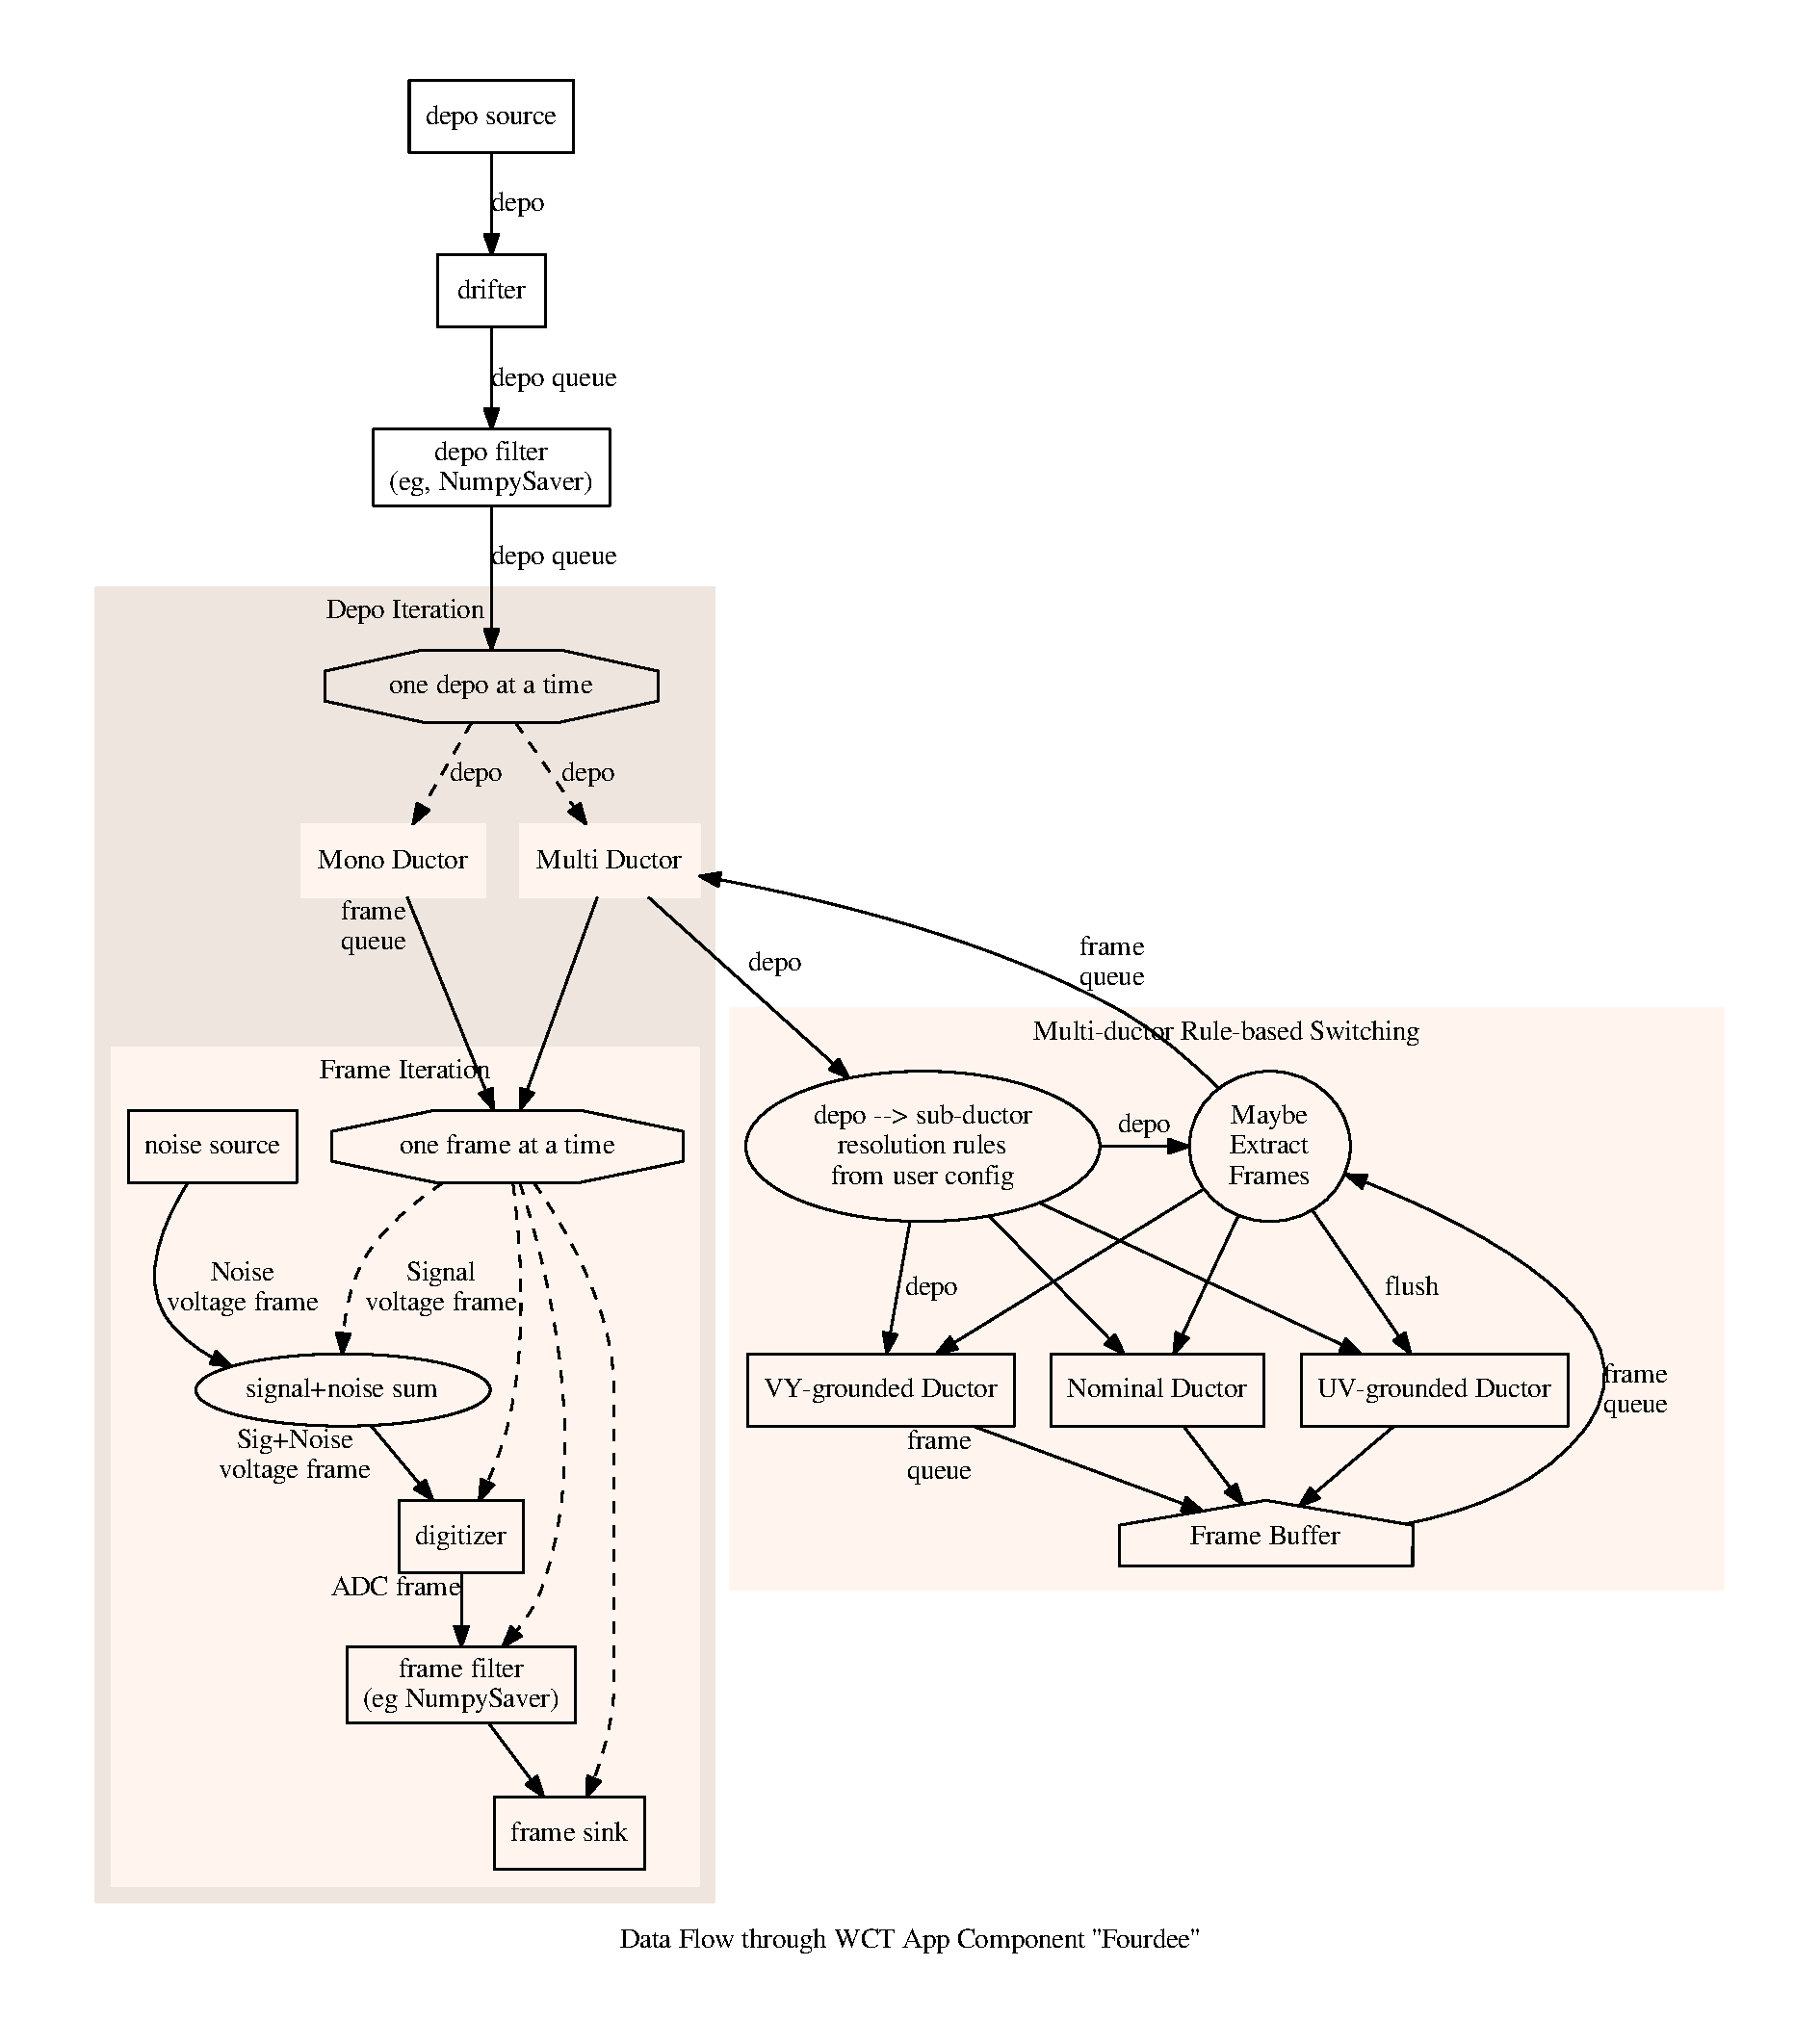
\includegraphics[height=4cm]{fourdee.pdf}

        \tiny hard-coded Fourdee structure
      \end{center}
    \end{column}
  \end{columns}

  \vspace{-10mm}

  
  \begin{center}
    \only<1>{signal + noise}
    \only<2>{just signal}

    \includegraphics<1>[width=\textwidth]{test_simgraph_noise.pdf}
    \includegraphics<2>[width=\textwidth]{test_simgraph_signal.pdf}

    {\scriptsize (generated directly from config)}
  \end{center}


  No longer need to develop new C++ ``app'' components just to change
  graph structure! 
  
\end{frame}

\begin{frame}
  \frametitle{Jsonnet External Variables}
  

  \begin{itemize}
  \item Jsonnet has function to ``inject'' an external variable.
  \item Can be used to implement  ``user visible'' switches.
    \begin{itemize}\scriptsize
    \item Currently we use it to switch ``configuration epochs''
      (before/after hardware fix) when compiling the
      \textit{.json.bz2} config files.
    \item[$|$] \texttt{local hwnf\_epoch = std.extVar("hwnf\_epoch");}
    \item[$|$] \texttt{if hwnf\_epoch == "before" then ...}
    \end{itemize}
  \item Inject from \texttt{wire-cell}, \texttt{jsonnet} command line programs:
    \begin{itemize}
    \item[ \$] \texttt{jsonnet -V hwnf\_epoch=before ...}
    \item[ \$] \texttt{wire-cell -V hwnf\_epoch=before ...}
    \end{itemize}
  \item Inject \textbf{from} \textit{art} FHiCL but no way to inject \textbf{to} FHiCL.
  \end{itemize}

\end{frame}

\section{NF Integration Issue}
\begin{frame}
  \tableofcontents[currentsection,hideothersubsections]
\end{frame}

\begin{frame}
  \frametitle{Configuration Epochs}
  WCT ``channel noise DB'' needs different configs (for ``RMS cut'')
  in pre- and post-hardware fix ``epochs''.
  \begin{itemize}\footnotesize
  \item Currently provide 2 pairs of WCT JSON and \textit{art} FHiCL config files.
  \item M. Kirby and Herb say two configs will lead to mistakes, want
    us to fix.
  \item No DB support, Mike says use hard-coded C++ switch on run number.
  \item But, WCT says, ``configure exactly once before data is processed!''
  \end{itemize}
  
\end{frame}
\begin{frame}
  \frametitle{Suggested Fix}
  \begin{enumerate}\footnotesize
  \item Develop new \textit{facacde} \texttt{ChannelNoiseDB} inside \texttt{larwirecell}
    \begin{itemize}\scriptsize
    \item It manages $N$ ``real'' \texttt{ChannelNoiseDB} instances.
    \end{itemize}
  \item Configuration associates a \textbf{run range} to each instance.
    \begin{itemize}\scriptsize
    \item Right now $N=2$: before/after.
    \item Each job creates and configures both \texttt{ChannelNoiseDB} instances.
    \end{itemize}
  \item The \textit{facade} \texttt{ChannelNoiseDB} IsA
    \texttt{IArtEventVisitor}:
    \begin{itemize}\scriptsize
    \item Can check run number on each event and then switch
      implementation when needed.
    \item Must check no WCT code caches some value from the CHNDB.
    \end{itemize}
  \end{enumerate}
  
\end{frame}
\end{document}

